\section{Resultados}

A metodologia descrita no corpo deste trabalho foi incorporada em linguagem de modelagem e aplicada à rede teórica em diferentes casos descritos a seguir.

\subsection{Rede de 45 barras}

Aplicou-se a técnica de reconfiguração para uma rede composta por 45 barras cuja topologia inicial é expressa pela figura~\ref{fig:45inicial}.
A rede possui tensão nominal no valor de \SI{13.8}{\kilo\volt} com alimentador no nó 1 e dados de impedâncias e corrente máxima expressas pela tabela~\ref{tab:imp}.
As chaves são representadas por quadriláteros, se preenchidas indicam chaves fechadas, do contrário chaves abertas.

\begin{table}[H]\tiny
    \caption{Parâmetros de impedância e corrente máxima para o conjunto de circuitos da rede didática de 45 nós}
    \label{tab:imp}
    \begin{minipage}{.5\linewidth}
        \centering
        \begin{tabular}{|c|c|c|c|c|}
        \hline
        $b_\text{part}$ & $b_\text{cheg}$& R [$\Omega$]  & X [$\Omega$] & Imax [A]\\ \hline
         2 &  3 & 0.0922 & 0.0470 & 200\\ \hline
         3 &  4 & 0.4930 & 0.2511 & 200\\ \hline
         4 &  5 & 0.3660 & 0.1864 & 200\\ \hline
         5 &  6 & 0.3811 & 0.1941 & 200\\ \hline
         6 &  7 & 0.8190 & 0.7070 & 200\\ \hline
         7 &  8 & 0.1872 & 0.6188 & 200\\ \hline
         9 & 10 & 0.7114 & 0.2351 & 200\\ \hline
        10 & 11 & 10.300 & 0.7400 & 200\\ \hline
        11 & 13 & 10.440 & 0.7400 & 200\\ \hline
        13 & 14 & 0.1966 & 0.0650 & 200\\ \hline
        14 & 15 & 0.3744 & 0.1238 & 200\\ \hline
        15 & 16 & 14.680 & 11.550 & 200\\ \hline
        17 & 18 & 0.5416 & 0.7129 & 200\\ \hline
        18 & 19 & 0.5910 & 0.5260 & 200\\ \hline
        19 & 20 & 0.7463 & 0.5450 & 200\\ \hline
        20 & 21 & 12.890 & 17.210 & 200\\ \hline
        21 & 22 & 0.7320 & 0.5740 & 200\\ \hline
         3 & 23 & 0.1640 & 0.1565 & 200\\ \hline        
        \end{tabular}
        
    \end{minipage}%
    \begin{minipage}{.5\linewidth}
        \centering
        \begin{tabular}{|c|c|c|c|c|}
        \hline
        $b_\text{part}$ & $b_\text{cheg}$& R [$\Omega$]  & X [$\Omega$] & Imax [A]\\ \hline    
        24 & 25 & 15.042 & 13.554 & 200\\ \hline
        25 & 26 & 0.4095 & 0.4784 & 200\\ \hline
        26 & 27 & 0.7089 & 0.9373 & 200\\ \hline
         4 & 30 & 0.4512 & 0.3083 & 200\\ \hline
        31 & 32 & 0.8980 & 0.7091 & 200\\ \hline
        32 & 33 & 0.8960 & 0.7011 & 200\\ \hline
         7 & 35 & 0.2030 & 0.1034 & 200\\ \hline
        36 & 37 & 0.2842 & 0.1447 & 200\\ \hline
        37 & 38 & 10.590 & 0.9337 & 200\\ \hline
        38 & 39 & 0.8042 & 0.7006 & 200\\ \hline
        39 & 40 & 0.5075 & 0.2585 & 200\\ \hline
        41 & 42 & 0.9744 & 0.9630 & 200\\ \hline
        42 & 43 & 0.3105 & 0.3619 & 200\\ \hline
        43 & 44 & 0.3410 & 0.5302 & 200\\ \hline
        10 & 28 & 20.000 & 20.000 & 200\\ \hline
        12 & 19 & 20.000 & 20.000 & 200\\ \hline
        18 & 29 & 20.000 & 20.000 & 200\\ \hline
        22 & 45 & 0.5000 & 0.5000 & 200\\ \hline
        34 & 39 & 0.5000 & 0.5000 & 200\\ \hline
        \end{tabular}
    \end{minipage} 
\end{table}

\begin{figure}[H]
    \centering
    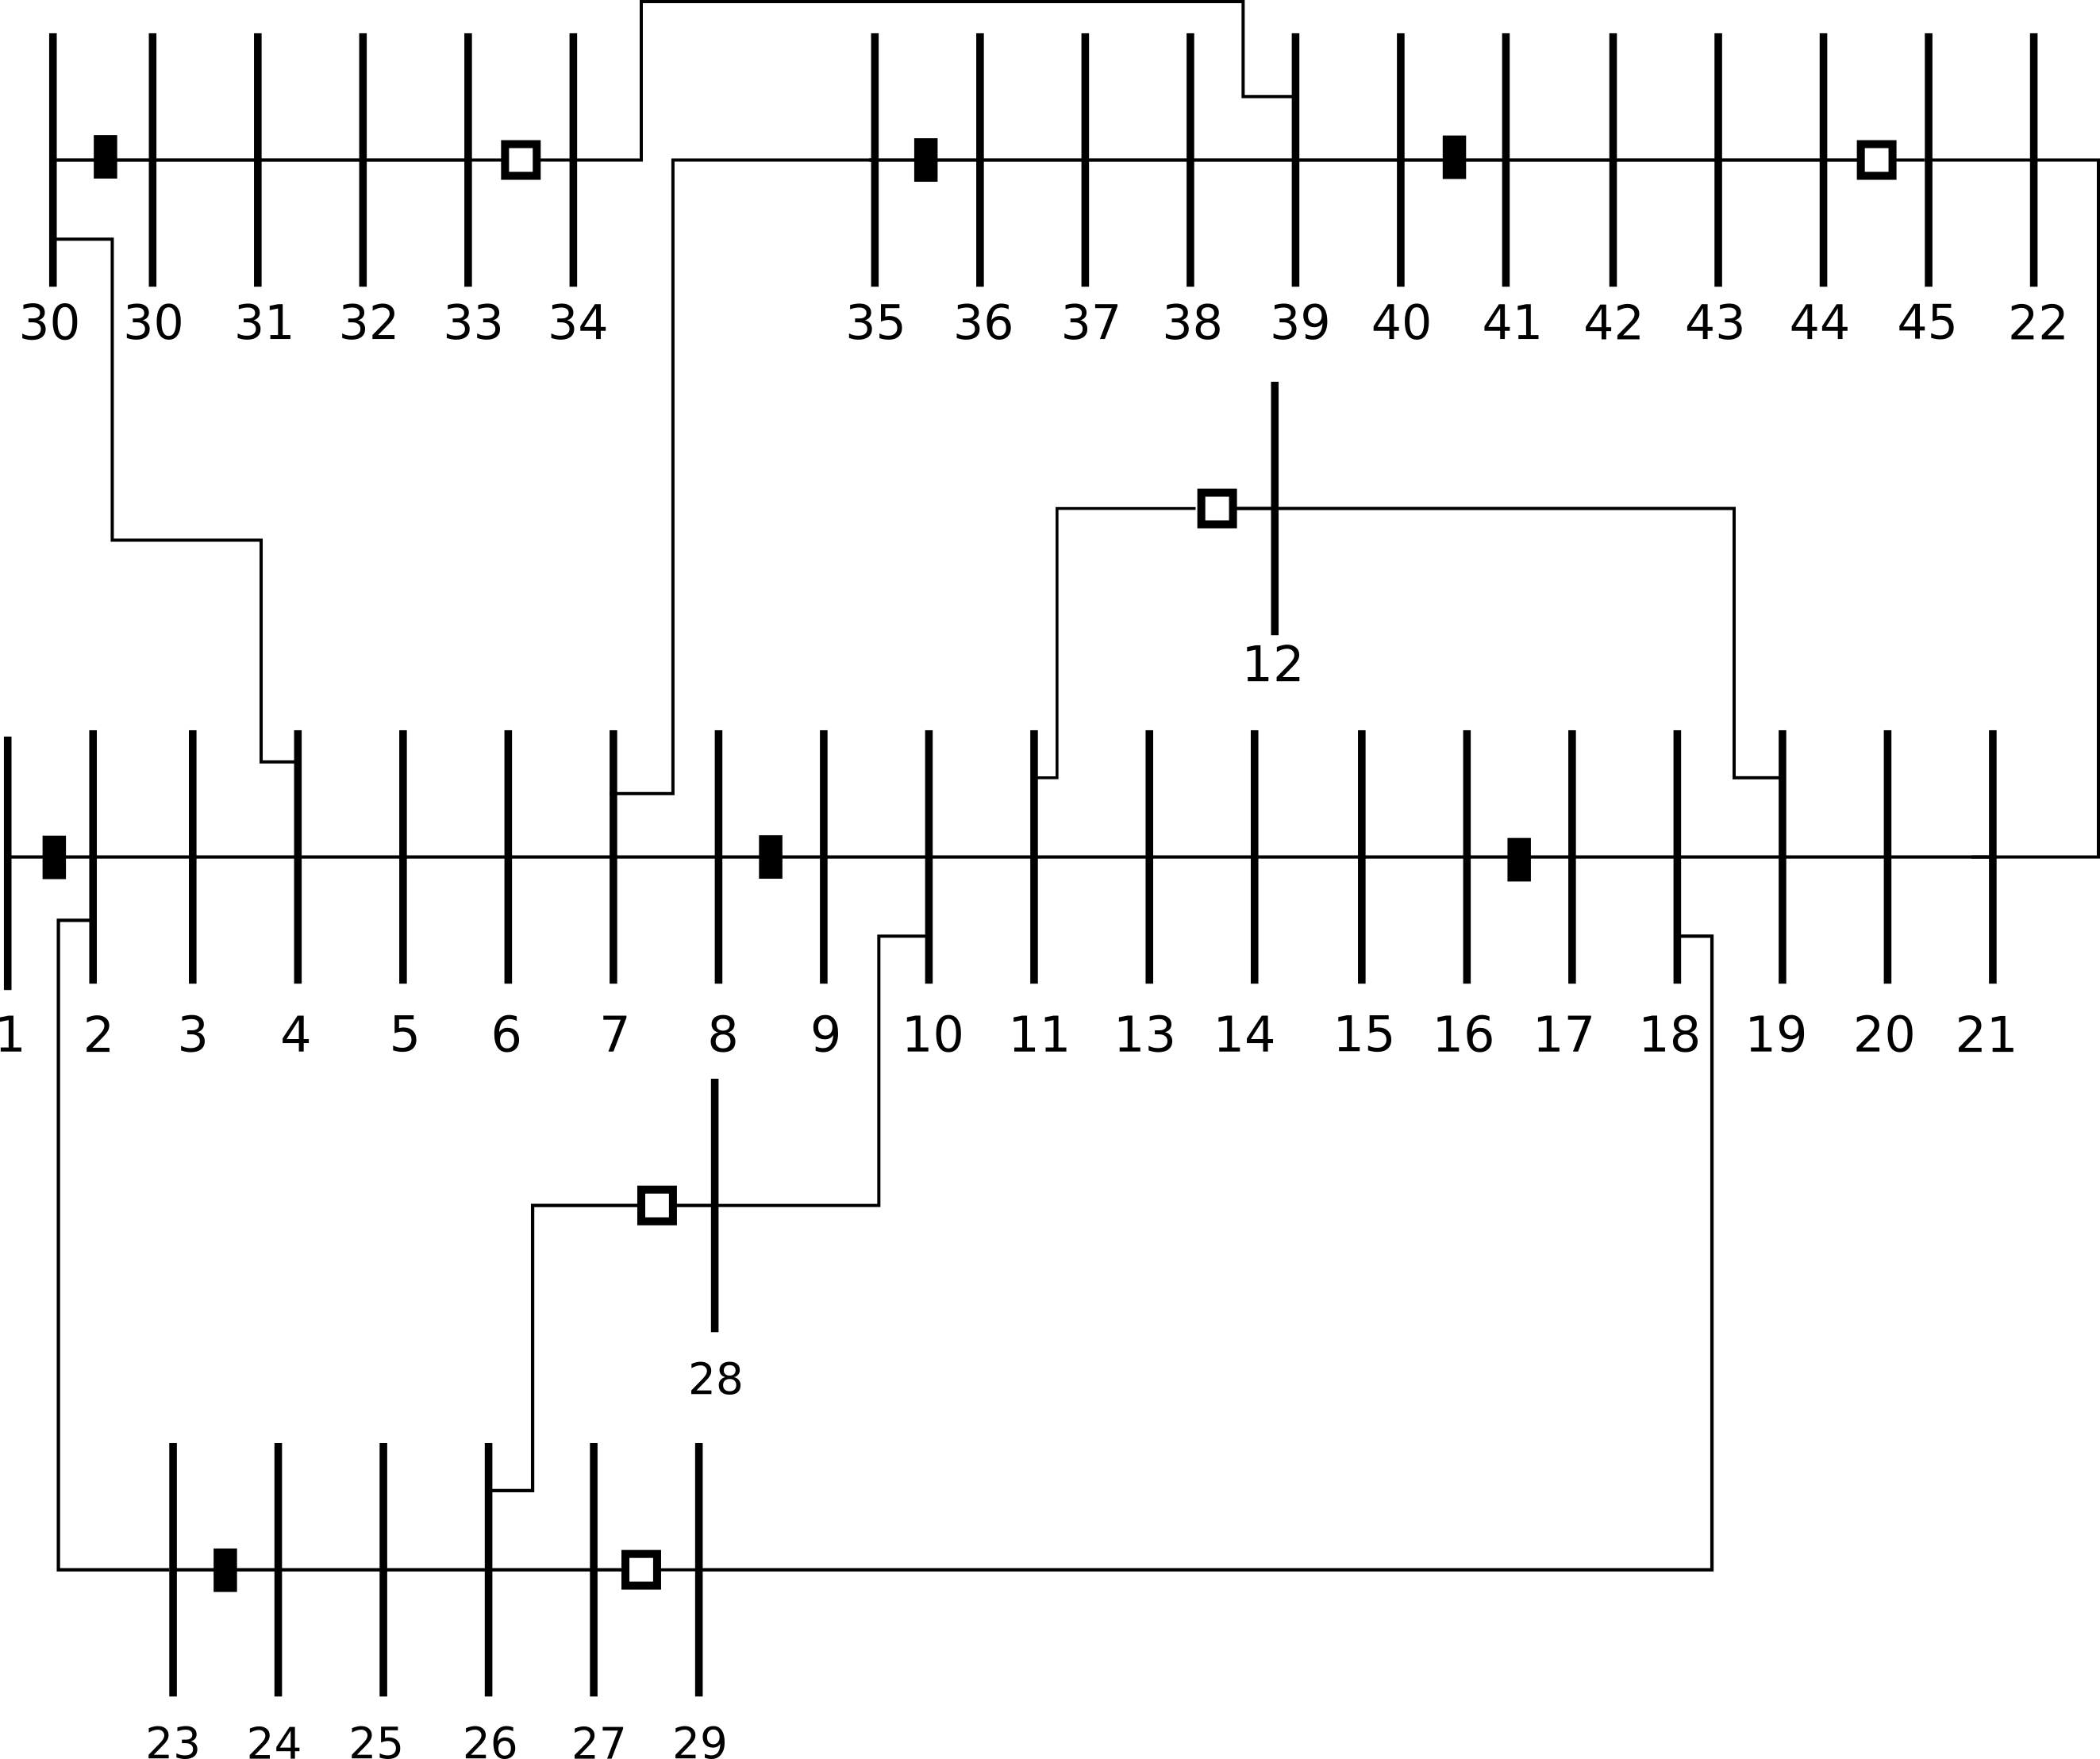
\includegraphics[width=0.6  \textwidth]{7_Results/img/rede_inicial.png}
    \caption{Topologia inicial da rede de 45 barras}
    \label{fig:45inicial}
\end{figure}



Nos perfis de demanda analisados a seguir, a topologia que minimiza as perdas ôhmicas é dada pela figura~\ref{fig:45final}.
Os resultados e discussões para os diferentes perfis de demanda podem ser vistos nas subseções seguintes.

\begin{figure}[H]
    \centering
    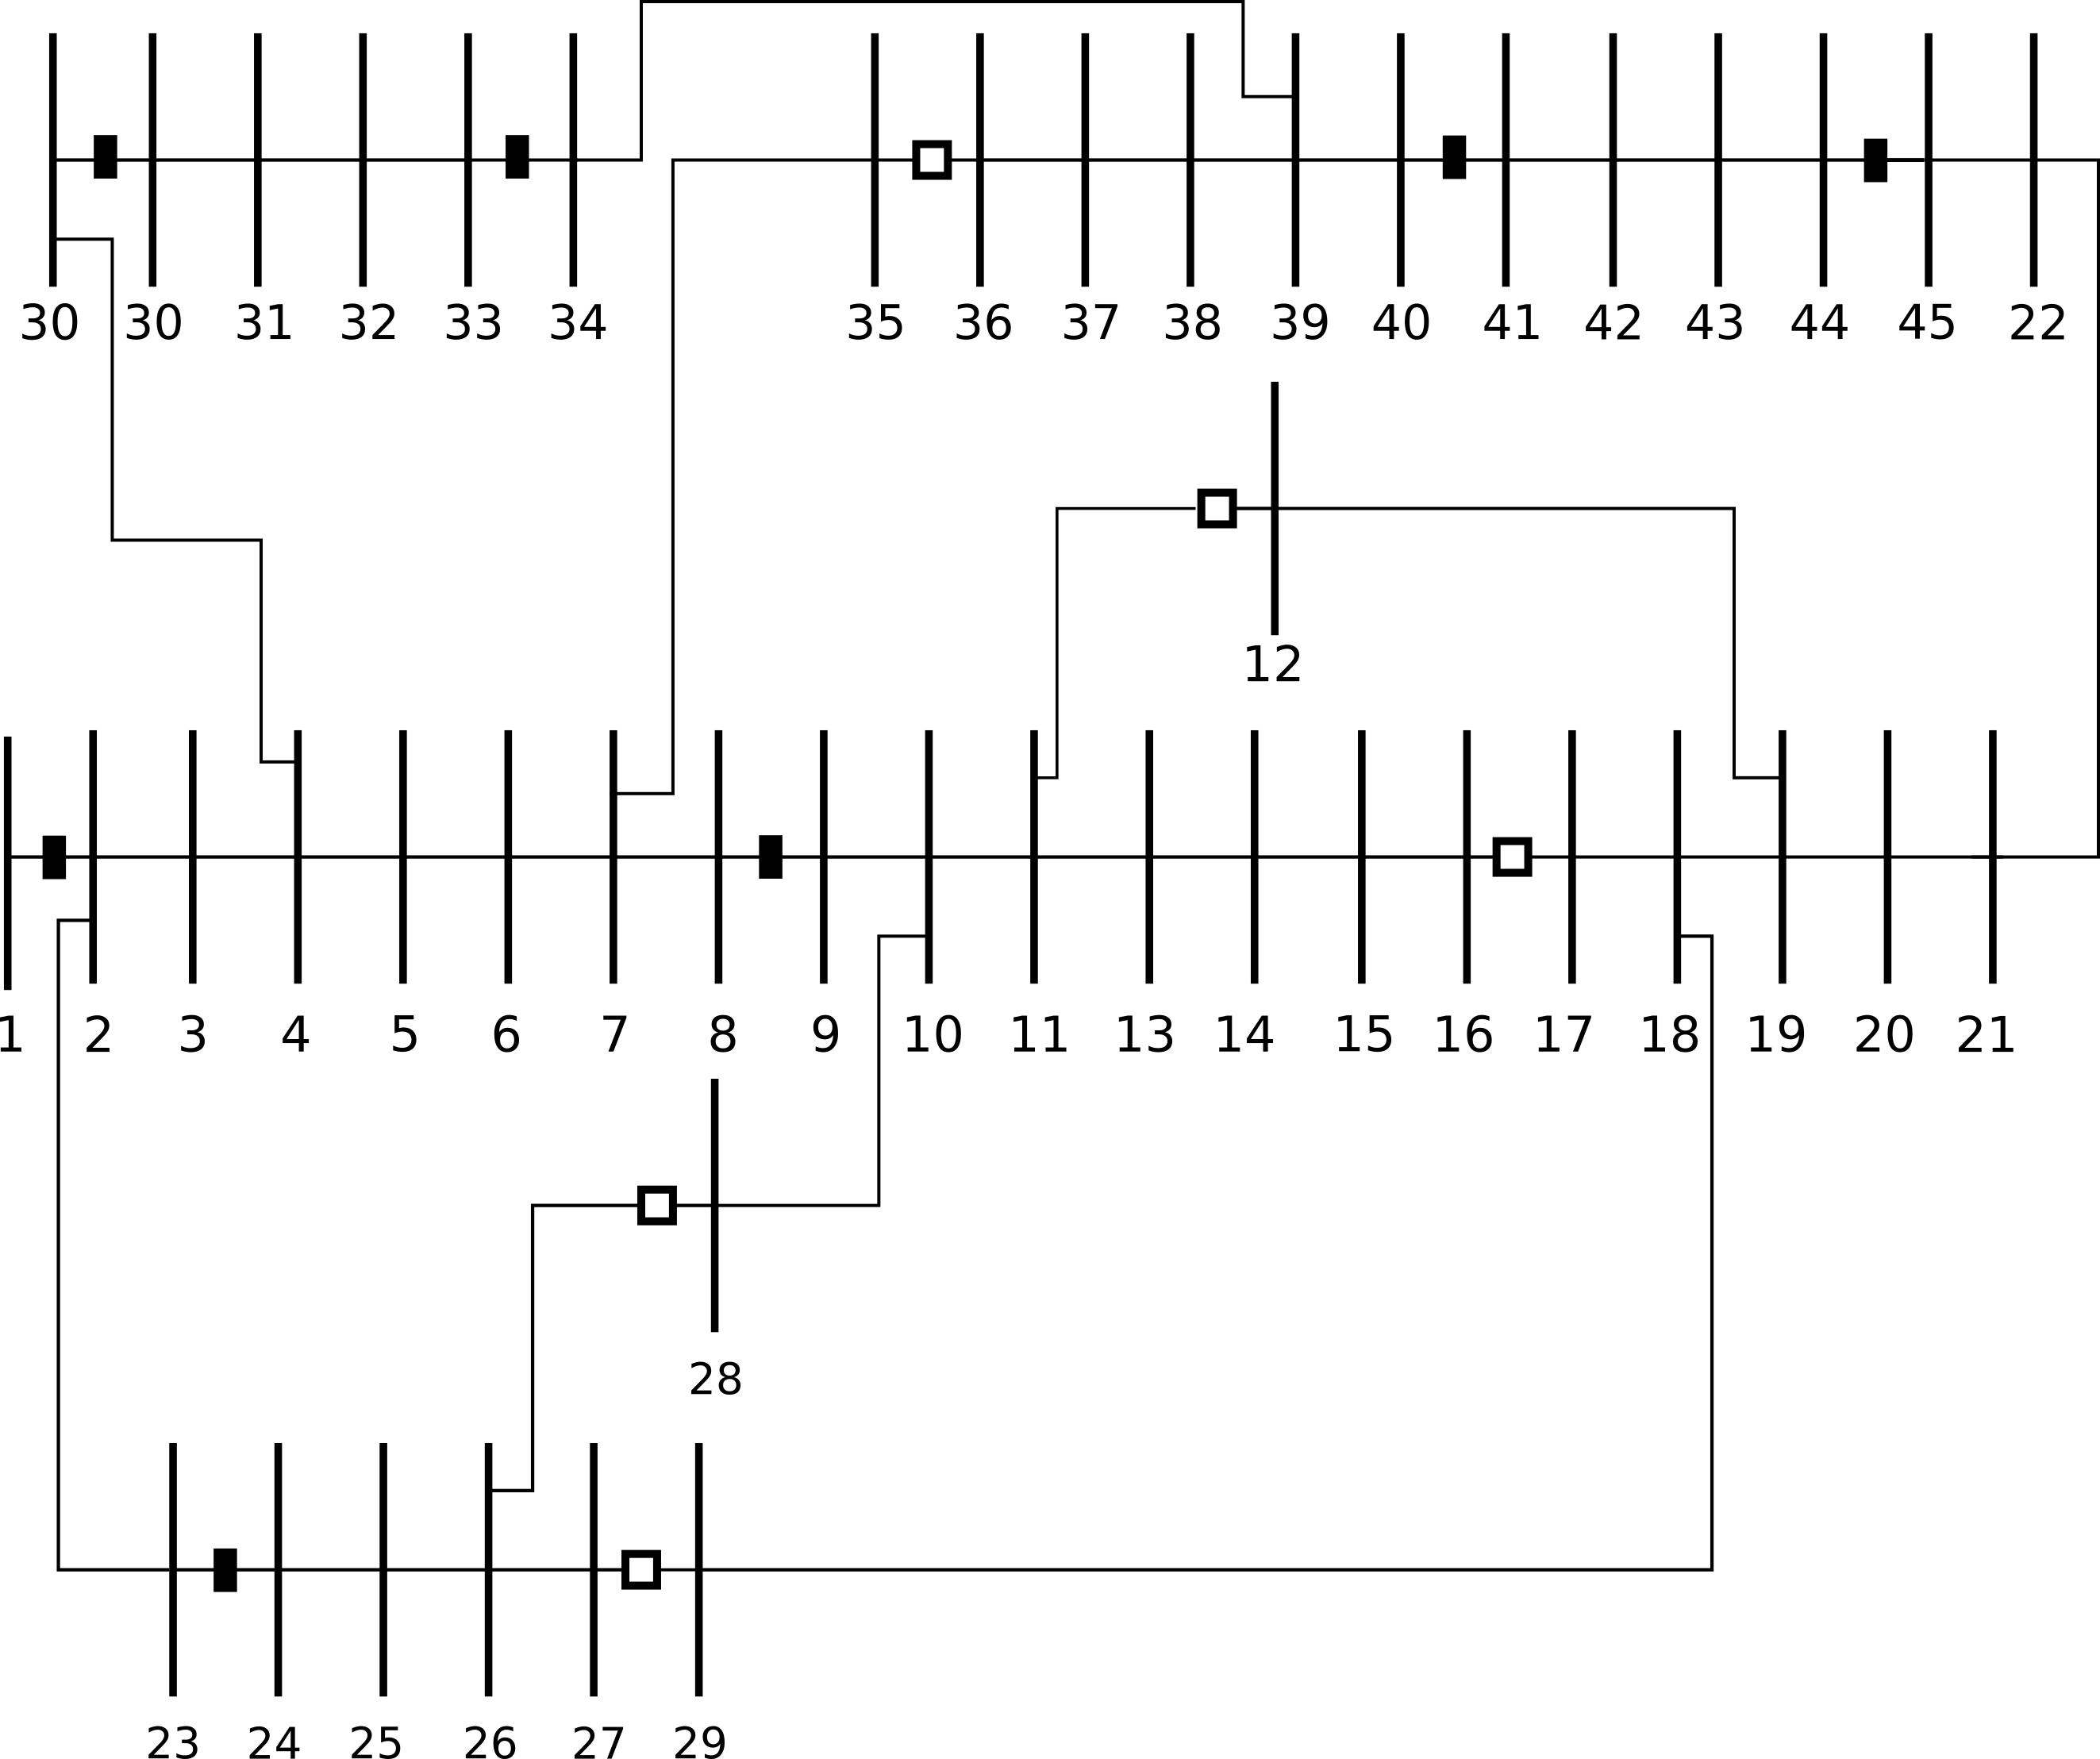
\includegraphics[width = 0.6\textwidth]{7_Results/img/rede_otimizada.png}
    \caption{Topologia da rede radial que minimiza as perdas ôhmicas}
    \label{fig:45final}
\end{figure}

\begin{table}[H]
    \centering
    \caption{Estado de operação das chaves antes e depois das configurações}
    \begin{tabular}{|c|c|c|c|}
    \hline
        i  &   j & Inicial & Reconfigurado\\ \hline
        1  &   2 & Fechado & Fechado\\ \hline
        8  &   9 & Fechado & Fechado\\ \hline                
        11 &  12 & Aberto  & Aberto \\ \hline   
        16 &  17 & Fechado & Aberto \\ \hline       
        23 &  24 & Fechado & Fechado \\ \hline       
        26 &  28 & Aberto  & Aberto \\ \hline            
        27 &  29 & Aberto  & Aberto\\ \hline            
        30 &  31 & Fechado & Fechado\\ \hline                
        33 &  34 & Aberto  & Fechado\\ \hline                
        35 &  36 & Fechado & Aberto\\ \hline                
        40 &  41 & Fechado & Fechado\\ \hline                    
        44 &  45 & Aberto  & Fechado\\ \hline
    \end{tabular}
    \label{tab:my_label}
\end{table}

\subsubsection{Demanda fixa}

O problema de reconfiguração da rede de 45 nós foi aplicado a uma demanda fixa cujos valores de potência ativa e reativa são expressas pelas figuras \ref{fig:45fixactive} e \ref{fig:45fixreactive} respectivamente.

\begin{figure}[H]
    \centering
    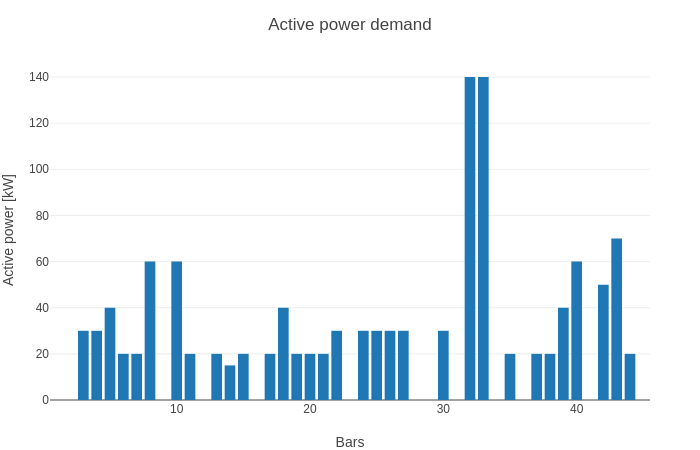
\includegraphics[width=0.7\textwidth]{7_Results/img/45fixdemand_active.png}
    \caption{Demanda de potência ativa por barra}
    \label{fig:45fixactive}
\end{figure}

\begin{figure}[H]
    \centering
    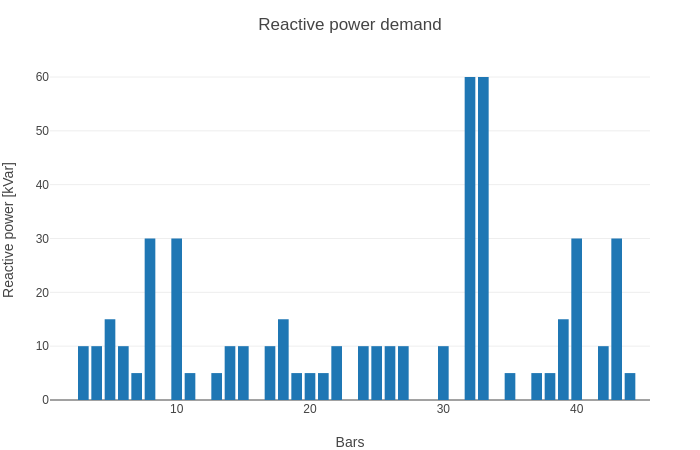
\includegraphics[width=0.7\textwidth]{7_Results/img/45fixdemand_reactive.png}
    \caption{Demanda de potência reativa por barra}
    \label{fig:45fixreactive}
\end{figure}

A partir da nova topologia, exibida na figura \ref{fig:45final}, os limites de tensões para as demandas das tabelas \ref{fig:45fixactive} e \ref{fig:45fixreactive} antes e depois da reconfiguração são dadas pelas figuras \ref{fig:45fixinitial} e \ref{fig:45fixafter} respectivamente.

\begin{figure}[H]
    \centering
    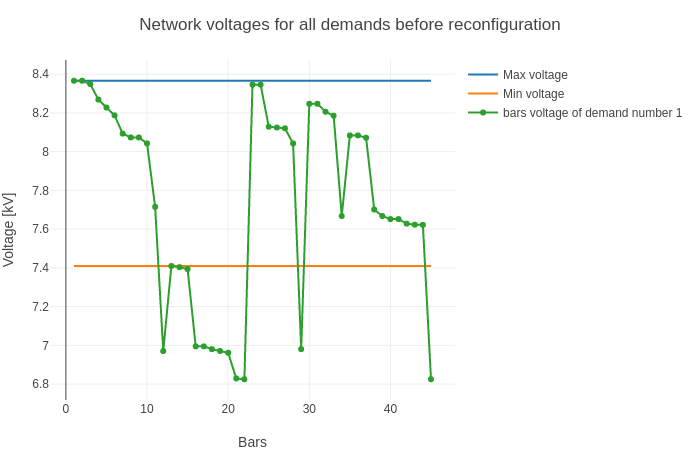
\includegraphics[width=\textwidth]{7_Results/img/45fixvoltages_before.png}
    \caption{Perfil de tensão para cada barra antes da reconfiguração}
    \label{fig:45fixinitial}
\end{figure}

\begin{figure}[H]
    \centering
    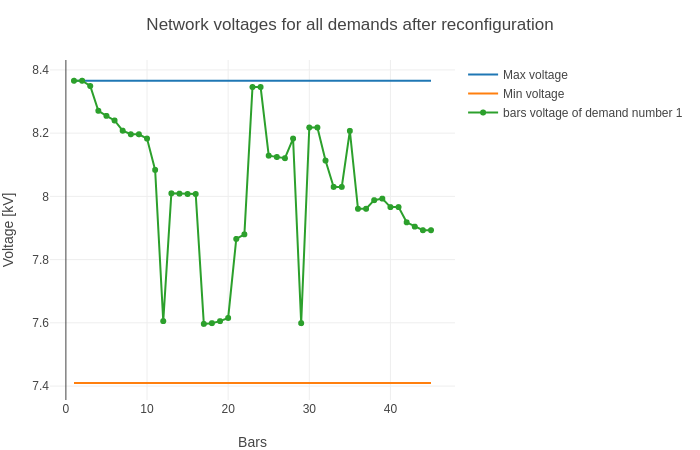
\includegraphics[width=\textwidth]{7_Results/img/45fixvoltages_after.png}
    \caption{Perfil de tensão para cada barra após a reconfiguração}
    \label{fig:45fixafter}
\end{figure}

Os dados gerais são para este perfil de demanda são dados pela tabela \ref{tab:resultsfixdemand}

\begin{table}[H]
    \centering
    \caption{Tabela de resultados para demanda fixa}
    \begin{tabular}{|c|c|c|}
    \hline
                                   & Inicial              & Reconfigurado               \\\hline
    Perdas ôhmicas por período       & \SI{613200.7}{\kilo\watt}      & \SI{369255.53}{\kilo\watt}  \\\hline
    Magnitude da tensão mínima     & \SI{6.82}{\kilo\volt}    & \SI{7.60}{\kilo\volt}   \\\hline
    Barra da tensão mínima         & 45                       & 17                      \\\hline
    Potência ativa da subestação   & \SI{1285.07}{\kilo\watt} & \SI{1257.17}{\kilo\watt}\\\hline
    Potência reativa da subestação & 495.00 kVar              & 495.17 kVar      \\\hline
    \end{tabular}
    \label{tab:resultsfixdemand}
\end{table}

Para um custo de US\$ 0.30 por kWh, o custo pré reconfiguração é de US\$ 183960,00 por ano em perdas, após a reconfiguração este custo é reduzido para US\$ 110776.00 por ano.

\subsubsection{Demanda com 3 níveis proporcionais}

\begin{figure}[H]
    \centering
    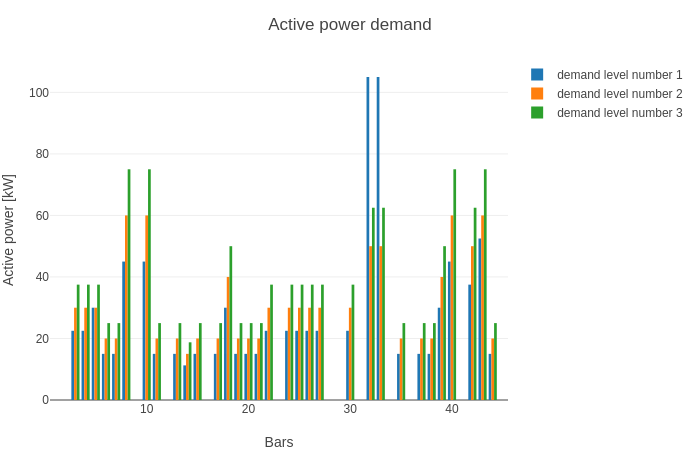
\includegraphics[width=0.8\textwidth]{7_Results/img/45demand_active.png}
    \caption{Demanda de potência ativa proporcionais a demanda média}
    \label{fig:45demandactive_propor}
\end{figure}

\begin{figure}[H]
    \centering
    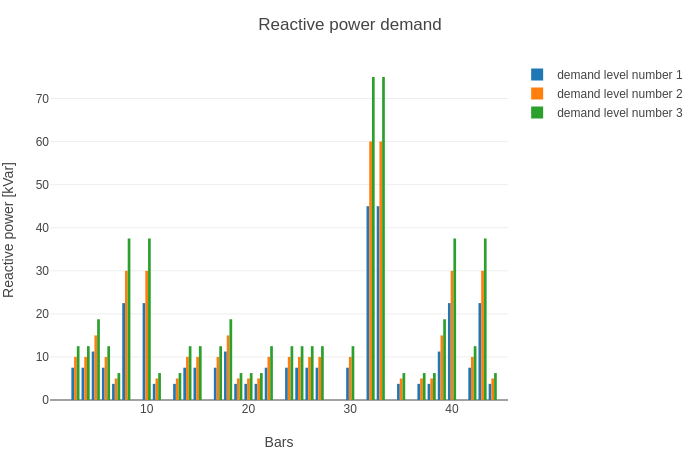
\includegraphics[width=0.8\textwidth]{7_Results/img/45demand_reactive.png}
    \caption{Demanda de potência ativa proporcionais a demanda média}
    \label{fig:45demandreactive_propor}
\end{figure}

\begin{figure}[H]
    \centering
    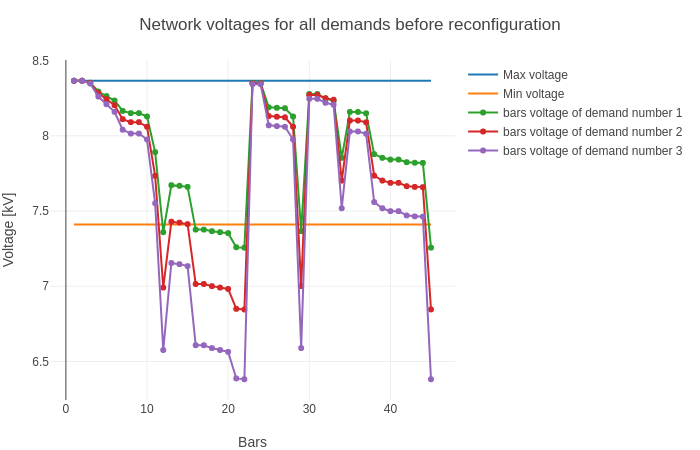
\includegraphics[width=0.8\textwidth]{7_Results/img/45voltages_before.png}
    \caption{Perfil de tensões para cada barra antes da reconfiguração}
    \label{fig:45voltages_beforesprop}
\end{figure}

\begin{figure}[H]
    \centering
    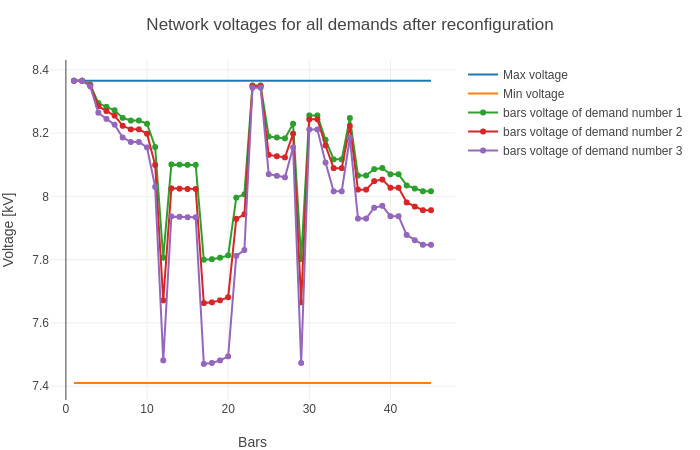
\includegraphics[width=0.8\textwidth]{7_Results/img/45voltages_after.png}
    \caption{Perfil de tensões para cada barra depois da reconfiguração}
    \label{fig:45voltaes_afterprop}
\end{figure}

\begin{table}[H]
    \centering
    \caption{Tabela de resultados para demanda 1}
    \begin{tabular}{|c|c|c|}
    \hline
                                   & Inicial              & Reconfigurado               \\\hline
    Perdas ôhmicas por período       & \SI{38768}{\kilo\watt\hour}      & \SI{23665}{\kilo\watt\hour}  \\\hline
    Magnitude da tensão mínima     & \SI{7.26}{\kilo\volt}    & \SI{7.8}{\kilo\volt}   \\\hline
    Barra da tensão mínima         & 45                       & 17                      \\\hline
    Potência ativa da subestação   & \SI{950}{\kilo\watt} & \SI{1257.17}{\kilo\watt}\\\hline
    Potência reativa da subestação & 495.00 kVar              & 495.17 kVar      \\\hline
    \end{tabular}
    \label{tab:45prop1}
\end{table}

\begin{table}[H]
    \centering
    \caption{Tabela de resultados para demanda 2}
    \begin{tabular}{|c|c|c|}
    \hline
                                   & Inicial              & Reconfigurado               \\\hline
    Perdas ôhmicas por período       & \SI{428788}{\kilo\watt\hour}      & \SI{217931}{\kilo\watt\hour}  \\\hline
    Magnitude da tensão mínima     & \SI{6.85}{\kilo\volt}    & \SI{7.66}{\kilo\volt}   \\\hline
    Barra da tensão mínima         & 45                       & 17                      \\\hline
    Potência ativa da subestação   & \SI{1078.4}{\kilo\watt} & \SI{1074.25}{\kilo\watt}\\\hline
    Potência reativa da subestação & 492.0 kVar              & 488.5 kVar      \\\hline
    \end{tabular}
    \label{tab:45prop2}
\end{table}

\begin{table}[H]
    \centering
    \caption{Tabela de resultados para demanda 3}
    \begin{tabular}{|c|c|c|}
    \hline
                                   & Inicial              & Reconfigurado               \\\hline
    Perdas ôhmicas por período       & \SI{100565.2}{\kilo\watt\hour}      & \SI{50693.4}{\kilo\watt\hour}  \\\hline
    Magnitude da tensão mínima     & \SI{6.38}{\kilo\volt}    & \SI{7.47}{\kilo\volt}   \\\hline
    Barra da tensão mínima         & 45                       & 17                      \\\hline
    Potência ativa da subestação   & \SI{1369.3}{\kilo\watt} & \SI{1319.46}{\kilo\watt}\\\hline
    Potência reativa da subestação & 624.0 kVar              & 618.3 kVar      \\\hline
    \end{tabular}
    \label{tab:45prop3}
\end{table}


Considerando um custo de US\$0.30 do kWh, antes da reconfiguração a rede, para o perfil de demanda analisado, gera um custo de aproximadamente US\$ 170436.00 devido à perdas ôhmicas em um período de 1 ano.
Após a reconfiguração, o custo devido às perdas ôhmicas é de US\$87867.00, este valor corresponde a uma redução de aproximadamente 48.5\% do valor inicial.

\subsubsection{Demanda com 4 níveis não proporcionais}

\begin{figure}[H]
    \centering
    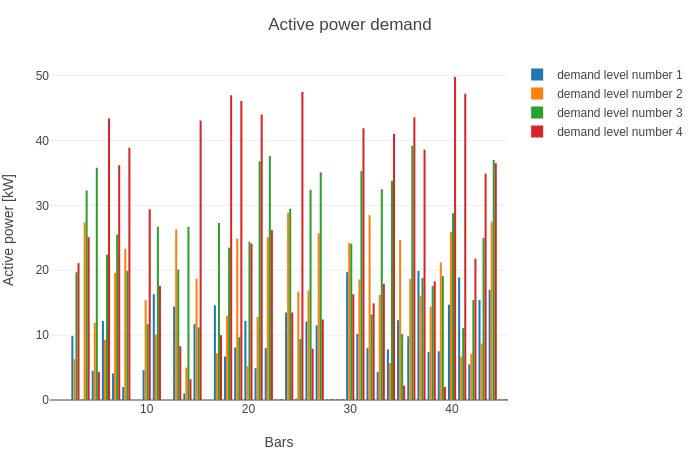
\includegraphics[width=0.8\textwidth]{7_Results/img/active_demand.png}
    \caption{Demanda de potência ativa do caso 2}
    \label{fig:45activepower2}
\end{figure}

\begin{figure}[H]
    \centering
    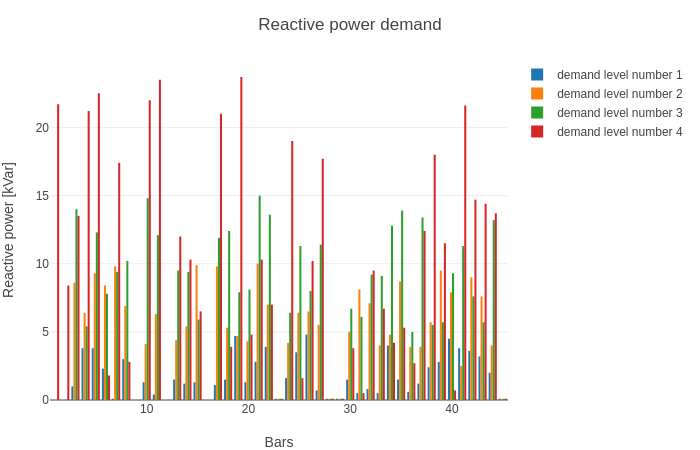
\includegraphics[width=0.7\textwidth]{7_Results/img/reactive_demand.png}
    \caption{Demanda de potência reativa do caso 2}
    \label{fig:45reactivepower2}
\end{figure}

\begin{figure}[H]
    \centering
    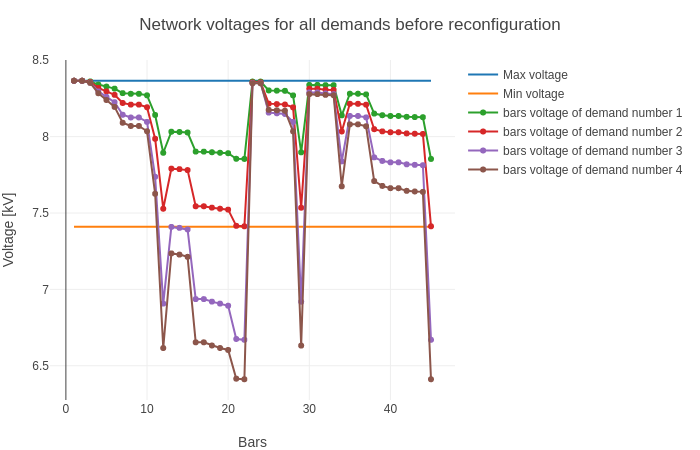
\includegraphics[width=0.9\textwidth]{7_Results/img/initial_voltages.png}
    \caption{Tensão nas barras da topologia inicial para demanda do caso 3}
    \label{fig:45voltages_init2}
\end{figure}

\begin{figure}[H]
    \centering
    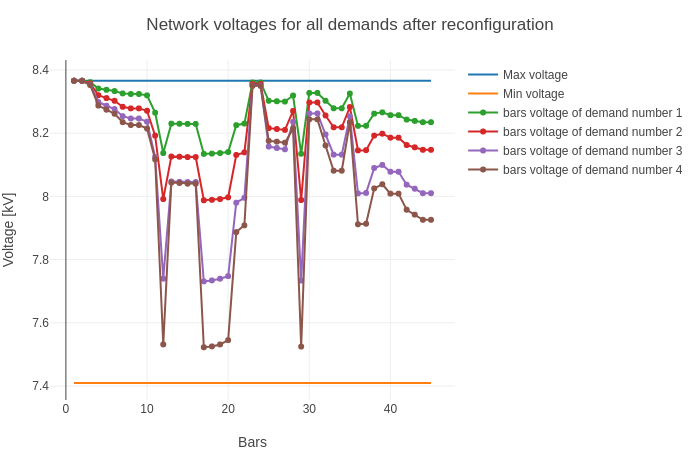
\includegraphics[width=0.9\textwidth]{7_Results/img/reconfig_voltages.png}
    \caption{Tensão nas barras após reconfiguração para demanda do caso 3}
    \label{fig:45voltages_reconfigured2}
\end{figure}

\begin{table}[H]
    \centering
    \caption{Tabela de resultados para demanda 1}
    \begin{tabular}{|c|c|c|}
    \hline
                                   & Inicial              & Reconfigurado               \\\hline
    Perdas ôhmicas por período       & \SI{7421.2}{\kilo\watt\hour}      & \SI{3817.15}{\kilo\watt\hour}  \\\hline
    Magnitude da tensão mínima     & \SI{7.85}{\kilo\volt}    & \SI{8.13}{\kilo\volt}   \\\hline
    Barra da tensão mínima         & 45                       & 17                      \\\hline
    Potência ativa da subestação   & \SI{359.9}{\kilo\watt} & \SI{355.8}{\kilo\watt}\\\hline
    Potência reativa da subestação & 82.0 kVar              & 82.0 kVar      \\\hline
    \end{tabular}
    \label{tab:45rand1}
\end{table}

\begin{table}[H]
    \centering
    \caption{Tabela de resultados para demanda 2}
    \begin{tabular}{|c|c|c|}
    \hline
                                   & Inicial              & Reconfigurado               \\\hline
    Perdas ôhmicas por período       & \SI{79273.2}{\kilo\watt\hour}      & \SI{39111.2}{\kilo\watt\hour}  \\\hline
    Magnitude da tensão mínima     & \SI{7.41}{\kilo\volt}    & \SI{7.99}{\kilo\volt}   \\\hline
    Barra da tensão mínima         & 45                       & 17                      \\\hline
    Potência ativa da subestação   & \SI{636.9}{\kilo\watt} & \SI{625.5}{\kilo\watt}\\\hline
    Potência reativa da subestação & 245.0 kVar              & 245.0 kVar      \\\hline
    \end{tabular}
    \label{tab:45rand2}
\end{table}

\begin{table}[H]
    \centering
    \caption{Tabela de resultados para demanda 3}
    \begin{tabular}{|c|c|c|}
    \hline
                                   & Inicial              & Reconfigurado               \\\hline
    Perdas ôhmicas por período       & \SI{99808.1}{\kilo\watt\hour}      & \SI{44325.2}{\kilo\watt\hour}  \\\hline
    Magnitude da tensão mínima     & \SI{6.67}{\kilo\volt}    & \SI{7.73}{\kilo\volt}   \\\hline
    Barra da tensão mínima         & 45                       & 17                      \\\hline
    Potência ativa da subestação   & \SI{936.2}{\kilo\watt} & \SI{904.5}{\kilo\watt}\\\hline
    Potência reativa da subestação & 375.0 kVar              & 370.0 kVar      \\\hline
    \end{tabular}
    \label{tab:45rand3}
\end{table}

\begin{table}[H]
    \centering
    \caption{Tabela de resultados para demanda 4}
    \begin{tabular}{|c|c|c|}
    \hline
                                   & Inicial              & Reconfigurado               \\\hline
    Perdas ôhmicas por período       & \SI{70956.8}{\kilo\watt\hour}      & \SI{32337.4}{\kilo\watt\hour}  \\\hline
    Magnitude da tensão mínima     & \SI{6.41}{\kilo\volt}    & \SI{7.52}{\kilo\volt}   \\\hline
    Barra da tensão mínima         & 45                       & 17                      \\\hline
    Potência ativa da subestação   & \SI{1057.6}{\kilo\watt} & \SI{1013.5}{\kilo\watt}\\\hline
    Potência reativa da subestação & 476.0 kVar              & 470.2 kVar      \\\hline
    \end{tabular}
    \label{tab:45rand4}
\end{table}

Com um custo de US\$ 0.30 para o kWh, para o perfil de demanda analisado, verifica-se um valor de US\$ 77237.80 antes da reconfiguração e US\$ 35877.29 para a nova topologia em um período de um ano.